\documentclass[12pt,a4paper]{article}

%------------------------------------------------------------
% Packages
%------------------------------------------------------------
\usepackage[utf8]{inputenc}
\usepackage[T5]{fontenc}
\usepackage[vietnamese,english]{babel}
\usepackage[top=2.5cm, bottom=2.5cm, left=2.5cm, right=2.5cm]{geometry}
\usepackage{times}
\usepackage{graphicx}
\usepackage{caption}
\usepackage{booktabs}
\usepackage{amsmath, amssymb}
\usepackage{multirow}
\usepackage{enumitem}
\usepackage{hyperref}
\usepackage{setspace}
\usepackage{titlesec}
\usepackage{fancyhdr}
\usepackage{array}
\usepackage{tabularx}
\usepackage{xcolor}
\usepackage{indentfirst}

\graphicspath{{figures/}}

%------------------------------------------------------------
% Page style
%------------------------------------------------------------
\pagestyle{fancy}
\fancyhf{}
\rhead{\thepage}
\lhead{\small Ước lượng công sức phần mềm bằng học máy đa lược đồ}
\setlength{\headheight}{14pt}

%------------------------------------------------------------
% Section formatting
%------------------------------------------------------------
\titleformat{\section}{\normalfont\bfseries\normalsize}{\thesection.}{0.5em}{}
\titleformat{\subsection}{\normalfont\bfseries\normalsize}{\thesubsection.}{0.5em}{}
\titlespacing{\section}{0pt}{12pt}{6pt}
\titlespacing{\subsection}{0pt}{8pt}{4pt}

\setlength{\parindent}{1.5em}
\onehalfspacing

%------------------------------------------------------------
% Document
%------------------------------------------------------------
\begin{document}

%------------------------------------------------------------
% TITLE BLOCK
%------------------------------------------------------------
\begin{center}
{\large\bfseries Khung Học Máy Kết Hợp Thống Nhất cho Ước Lượng Công Sức Phần Mềm Trên Nhiều Lược Đồ Đo Lường}\\[4pt]
{\normalsize\bfseries A Unified Ensemble Learning Framework for Software Effort Estimation Across Multiple Schemas}\\[10pt]

{\normalsize
Nguyễn Nhật Huy, Nguyễn Đức Mạn, Đặng Nhật Minh, Nguyễn Thúy Giang\\[4pt]
}

{\small\itshape
$^{a}$Chương trình Công Nghệ Phần Mềm Việt Mỹ CMU~--~Khoa Đào Tạo Quốc Tế,\\
Đại học Duy Tân, Đà Nẵng, Việt Nam\\[4pt]
}

{\normalsize\bfseries GVHD: Ph.D P.W.C. Prasad, Ph.D Md Shohel Sayeed}
\end{center}

\vspace{8pt}
\hrule
\vspace{6pt}

%------------------------------------------------------------
% ABSTRACT (TÓM TẮT)
%------------------------------------------------------------
\noindent\textbf{Tóm tắt}

\vspace{4pt}
\noindent
Ước lượng công sức phần mềm chính xác trên nhiều loại dự án khác nhau là bài toán khó khăn bởi các điểm chuẩn hiện có thiếu tính minh bạch về nguồn gốc dữ liệu, sử dụng mô hình tham số chưa hiệu chỉnh và báo cáo kết quả tổng hợp che giấu hành vi theo từng lược đồ. Nghiên cứu này đề xuất một khung thống nhất, có thể tái lập, bao phủ ba lược đồ đo kích thước: Dòng mã lệnh (Lines of Code -- LOC), Điểm chức năng (Function Points -- FP) và Điểm trường hợp sử dụng (Use Case Points -- UCP). Chúng tôi đánh giá năm mô hình học máy -- Hồi quy tuyến tính, Cây quyết định, Rừng ngẫu nhiên, Tăng cường độ dốc và XGBoost -- trên 3.054 dự án từ 18 nguồn công khai (1979--2022). Rừng ngẫu nhiên đạt hiệu suất tốt nhất: MAE~$= 12{,}66 \pm 0{,}85$ người-tháng, MMRE~$= 0{,}647 \pm 0{,}041$, PRED(25)~$= 0{,}395$ -- cải thiện 42\% MMRE so với mô hình cơ sở đã hiệu chỉnh (MMRE~$= 1{,}12 \pm 0{,}08$). Kiểm định bỏ-một-nguồn (LOSO) chỉ cho thấy suy giảm MAE 21\%, xác nhận khả năng tổng quát hóa qua nhiều nguồn dữ liệu. Đóng góp chính của nghiên cứu là phương pháp luận chuẩn hóa: khung đánh giá tái lập, theo lược đồ, nhận thức mất cân bằng với mã nguồn mở và tập lệnh tái tạo dữ liệu.

\vspace{6pt}
\noindent\textbf{Từ khóa:} Ước lượng công sức; học máy; kỹ thuật phần mềm; lược đồ LOC, FP, UCP; Rừng ngẫu nhiên; chuẩn hóa đa lược đồ; tái lập kết quả nghiên cứu.

\vspace{4pt}
\hrule
\vspace{10pt}

%------------------------------------------------------------
% SECTION 1: MỞ ĐẦU
%------------------------------------------------------------
\section{Mở đầu}

Ước lượng công sức phát triển phần mềm là yếu tố then chốt quyết định sự thành công của các dự án phần mềm. Ước lượng chính xác hỗ trợ lập kế hoạch hiệu quả, phân bổ ngân sách, nguồn lực và quản lý rủi ro. Ngược lại, ước lượng sai thường dẫn đến vượt chi phí, trễ tiến độ, thậm chí thất bại dự án -- điều được ghi nhận rộng rãi trong tài liệu kỹ thuật phần mềm thực nghiệm.

Theo nhiều nghiên cứu, hơn 60\% dự án phần mềm gặp sự cố liên quan đến ước lượng không chính xác, với tỷ lệ vượt chi phí trung bình từ 30\% đến 200\% so với kế hoạch ban đầu. Sự đa dạng ngày càng tăng của các dự án phần mềm hiện đại -- khác biệt về kích thước, phương pháp, lĩnh vực và cấu trúc nhóm -- khiến việc tạo ra ước lượng nhất quán và đáng tin cậy ngày càng trở nên phức tạp.

Các mô hình tham số truyền thống như COCOMO~II cung cấp tính minh bạch thông qua công thức đóng và đã được áp dụng rộng rãi trong môi trường công nghiệp. Tuy nhiên, dạng hàm cố định của chúng gặp khó khăn trong việc tổng quát hóa trên các tập dữ liệu hiện đại đa dạng. Điều này thúc đẩy việc khám phá các phương pháp học máy linh hoạt hơn, có khả năng nắm bắt các mẫu phi tuyến và thích nghi với nhiều đặc điểm dự án khác nhau.

Dự án này, \textbf{``Khung Học Máy Kết Hợp Thống Nhất cho Ước Lượng Công Sức Phần Mềm''}, được đề xuất nhằm giải quyết ba vấn đề cốt lõi còn tồn đọng trong lĩnh vực: (i) thiếu tính kiểm toán về nguồn gốc dữ liệu, (ii) so sánh không công bằng với mô hình tham số chưa hiệu chỉnh, và (iii) báo cáo kết quả tổng hợp không rõ ràng che giấu hành vi theo lược đồ riêng biệt.

Hệ thống hỗ trợ đánh giá trên ba lược đồ đo lường chính: LOC (11 nguồn, 2.765 dự án), FP (4 nguồn, 158 dự án) và UCP (3 nguồn, 131 dự án). Về mặt kỹ thuật, khung được xây dựng bằng Python với các thư viện Scikit-learn, XGBoost và SciPy, áp dụng kiểm định thống kê Wilcoxon và hiệu chỉnh Holm-Bonferroni để đảm bảo độ tin cậy của kết quả.

%------------------------------------------------------------
% SECTION 2: TỔNG QUAN
%------------------------------------------------------------
\section{Tổng quan tình hình nghiên cứu}

\subsection{Tổng quan tình hình nghiên cứu}

Trong những thập kỷ gần đây, ước lượng công sức phần mềm đã thu hút sự quan tâm nghiên cứu đáng kể, đặc biệt là việc ứng dụng các kỹ thuật học máy để cải thiện độ chính xác so với các mô hình tham số truyền thống.

Các mô hình tham số như COCOMO (Constructive Cost Model) và COCOMO~II~\cite{boehm2000cocomo} đã được áp dụng rộng rãi kể từ những năm 1980. Những mô hình này dự đoán công sức dựa trên các thước đo kích thước phần mềm (LOC, FP) và các nhân tố chi phí. Tuy nhiên, hình thức hàm cố định của chúng thường không khái quát hóa tốt trên các tập dữ liệu đa dạng hiện đại, và việc áp dụng với các tham số mặc định khi thiếu dữ liệu chi phí tạo ra các so sánh không công bằng.

Nhiều nghiên cứu gần đây đã cho thấy các phương pháp học máy, đặc biệt là mô hình kết hợp (ensemble), có thể cải thiện đáng kể độ chính xác ước lượng. Rừng ngẫu nhiên (Random Forest) và Tăng cường độ dốc (Gradient Boosting) liên tục vượt trội hơn các phương pháp đơn lẻ trên nhiều tập dữ liệu riêng lẻ~\cite{tanveer2023survey}. Các nghiên cứu học sâu~\cite{azzeh2019cross} đã khám phá mạng LSTM và Transformer cho bài toán ước lượng, mặc dù những phương pháp này thường gặp vấn đề quá khớp khi dữ liệu hạn chế.

Tuy nhiên, ba vấn đề nghiêm trọng thường hạn chế độ mạnh và khả năng tái lập của các kết quả được báo cáo:

\begin{itemize}[leftmargin=2em]
    \item \textbf{Tính kiểm toán yếu} của các tập dữ liệu tổng hợp: nguồn gốc, quy tắc loại trùng lặp và khả năng tái tạo thường không rõ ràng.
    \item \textbf{Mô hình cơ sở không công bằng hoặc không thể tái lập}: COCOMO~II thường được áp dụng với tham số tùy ý khi thiếu dữ liệu chi phí, tạo ra so sánh kiểu ``bù nhìn rơm''.
    \item \textbf{Báo cáo ``tổng thể'' mơ hồ}: tổng hợp đa lược đồ có thể bị chi phối bởi lược đồ lớn nhất (thường là LOC), che giấu hành vi thực sự trên FP/UCP.
\end{itemize}

Theo thống kê từ các khảo sát hệ thống, hơn 75\% nghiên cứu ước lượng công sức chỉ báo cáo kết quả tổng hợp mà không phân tách theo lược đồ đo lường, làm giảm tính hữu ích thực tiễn của các kết quả này.

\begin{figure}[htbp]
\centering
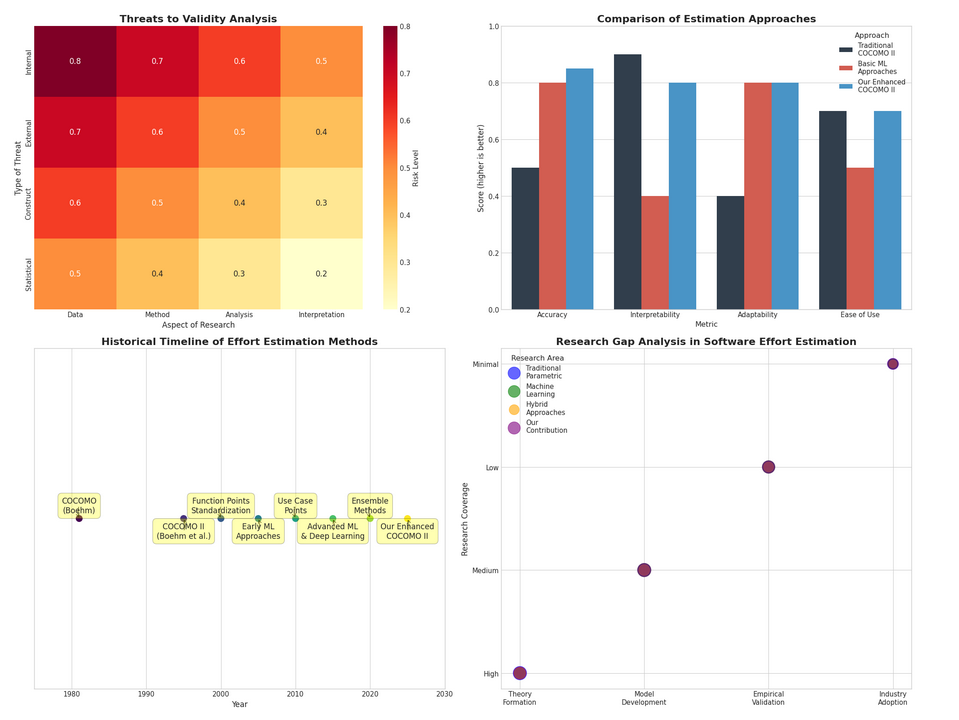
\includegraphics[width=0.90\linewidth]{related_work}
\caption{Tổng quan các phương pháp ước lượng công sức phần mềm trong tài liệu nghiên cứu: từ mô hình tham số đến học máy kết hợp và học sâu.}
\label{fig:related-work}
\end{figure}

\subsection{Đánh giá chung}

Các nghiên cứu về ước lượng công sức phần mềm cho thấy sự quan tâm ngày càng tăng đối với các phương pháp học máy, đặc biệt là mô hình kết hợp. Nhiều nền tảng và công cụ đã được phát triển nhằm hỗ trợ quá trình ước lượng và so sánh mô hình.

Tuy nhiên, phần lớn các nghiên cứu vẫn tập trung vào một lược đồ đơn lẻ (thường là LOC) và không cung cấp tập lệnh tái tạo dữ liệu hay bảng kê khai nguồn gốc đầy đủ. Sự thiếu hụt của các giao thức đánh giá đa lược đồ tích hợp và chuẩn hóa là khoảng trống nghiên cứu rõ ràng mà công trình này hướng đến giải quyết.

Do đó, dự án \textbf{Khung Học Máy Kết Hợp Thống Nhất} được đề xuất nhằm phát triển một khung đánh giá tái lập, theo lược đồ, nhận thức mất cân bằng với bảng kê khai dữ liệu mở và tập lệnh tái tạo, cung cấp mẫu chuẩn cho các nghiên cứu ước lượng công sức phần mềm trong tương lai.

%------------------------------------------------------------
% SECTION 3: ĐỀ XUẤT
%------------------------------------------------------------
\section{Đề xuất}

Nhằm giải quyết các hạn chế nêu trên, nhóm nghiên cứu đề xuất một khung đánh giá học máy thống nhất cho bài toán ước lượng công sức phần mềm trên ba lược đồ đo lường. Hệ thống cho phép người dùng tải dữ liệu từ 18 nguồn công khai, thực hiện tiền xử lý chuẩn hóa, huấn luyện và so sánh năm mô hình học máy, đồng thời đánh giá kết quả theo từng lược đồ và tổng hợp macro-average.

Để đạt được mục tiêu này, nhóm nghiên cứu đề xuất bốn giải pháp chính:

\begin{enumerate}[leftmargin=2em]
    \item \textbf{Bảng kê khai dữ liệu có kiểm toán:} Xây dựng bảng kê khai toàn diện 18 nguồn dữ liệu với thông tin nguồn gốc, DOI/URL, số lượng thô, quy tắc loại trùng lặp và tập lệnh tái tạo đầy đủ.
    \item \textbf{Mô hình cơ sở tham số công bằng:} Áp dụng mô hình lũy thừa hiệu chỉnh theo từng lược đồ và seed ngẫu nhiên để so sánh công bằng khi thiếu dữ liệu nhân tố chi phí.
    \item \textbf{Giao thức đánh giá theo lược đồ:} Sử dụng phân tầng 80/20 với kiểm định chéo 5-fold cho LOC/UCP và LOOCV cho FP, báo cáo riêng biệt và tổng hợp macro-average.
    \item \textbf{Phân tích loại bỏ thành phần (Ablation):} Định lượng đóng góp của từng bước tiền xử lý và kiểm định thống kê Wilcoxon với hiệu chỉnh Holm-Bonferroni.
\end{enumerate}

\subsection{Đề xuất công nghệ}

Để xây dựng khung học máy cho ước lượng công sức phần mềm, nhóm nghiên cứu sử dụng các công nghệ sau:

\textbf{Ngôn ngữ lập trình và thư viện ML:}
Python là ngôn ngữ chính, sử dụng các thư viện Scikit-learn~\cite{virtanen2020scipy} cho các mô hình học máy cơ bản (Hồi quy tuyến tính, Cây quyết định, Rừng ngẫu nhiên, Tăng cường độ dốc), XGBoost~\cite{chen2016xgboost} cho mô hình kết hợp nâng cao, SciPy để tối ưu hóa phi tuyến cho mô hình cơ sở lũy thừa, NumPy và Pandas để xử lý dữ liệu, và Matplotlib/Seaborn để trực quan hóa kết quả.

\textbf{Mô hình học máy được đánh giá:}
\begin{itemize}[leftmargin=2em]
    \item \textbf{Hồi quy tuyến tính (Linear Regression):} Bao gồm biến thể log-log để nắm bắt quan hệ nhân tử.
    \item \textbf{Cây quyết định (Decision Tree):} Độ sâu tối đa 10; nắm bắt tương tác phi tuyến.
    \item \textbf{Rừng ngẫu nhiên (Random Forest):} 100 cây ước lượng, độ sâu tối đa 15; phương pháp kết hợp mạnh mẽ.
    \item \textbf{Tăng cường độ dốc (Gradient Boosting):} 100 ước lượng, tốc độ học 0,1; xây dựng mô hình tuần tự.
    \item \textbf{XGBoost:} 100 ước lượng, độ sâu tối đa 5; chính quy hóa L1/L2 tích hợp.
\end{itemize}

\textbf{Giao thức kiểm định:}
Với LOC và UCP: phân chia 80/20 có phân tầng với kiểm định chéo 5-fold bên trong cho điều chỉnh siêu tham số. Với FP: Leave-One-Out Cross-Validation do kích thước mẫu giới hạn ($n=158$). Tất cả thực nghiệm được lặp lại với 10 seed ngẫu nhiên (1, 11, 21, \ldots, 91) để đánh giá độ ổn định.

\textbf{Cơ sở dữ liệu:}
Dữ liệu từ 18 nguồn công khai được lưu trữ dưới dạng CSV có phiên bản, với bảng kê khai đầy đủ bao gồm MD5 hash để đảm bảo tính toàn vẹn và tái tạo độc lập.

\subsection{Phương pháp giải quyết vấn đề}

Nghiên cứu này đề xuất một phương pháp luận bốn bước để giải quyết bài toán ước lượng công sức phần mềm đa lược đồ:

\textbf{Bước 1 -- Thu thập và phân vùng dữ liệu:} Tổng hợp 3.054 dự án từ 18 nguồn độc lập (1979--2022), phân vùng theo lược đồ đo lường (LOC: 2.765 dự án; FP: 158 dự án; UCP: 131 dự án). Thực hiện loại trùng lặp bảo thủ dựa trên khớp tên dự án chuẩn hóa, kích thước và công sức, loại bỏ 7,2\% bản ghi trùng lặp (236 trên 3.290).

\textbf{Bước 2 -- Tiền xử lý toàn diện:} Áp dụng pipeline 5 bước độc lập cho từng lược đồ: (i) chuẩn hóa đơn vị (công sức về người-tháng, LOC về KLOC); (ii) xử lý giá trị thiếu bằng điền median; (iii) giới hạn ngoại lệ dựa trên IQR ($1{,}5\times$ IQR); (iv) biến đổi log với $\log1p(x)$ để giảm độ lệch; (v) chuẩn hóa đặc trưng về phạm vi $[0, 1]$.

\textbf{Bước 3 -- Huấn luyện với kiểm định chéo lồng nhau:} Với mỗi lược đồ và 10 seed ngẫu nhiên, thực hiện pipeline huấn luyện hoàn chỉnh. Mô hình cơ sở lũy thừa $E = A \times (\text{Kích thước})^B$ được hiệu chỉnh bằng bình phương tối thiểu phi tuyến, đảm bảo so sánh công bằng dựa trên cùng dữ liệu huấn luyện.

\textbf{Bước 4 -- Đánh giá đa chỉ số và kiểm định thống kê:} Tính 7 chỉ số chuẩn (MMRE, MdMRE, PRED(25), MAE, MdAE, RMSE, $R^2$), tổng hợp bằng macro-average (mỗi lược đồ đóng góp bằng nhau), và kiểm định Wilcoxon với hiệu chỉnh Holm-Bonferroni ở $\alpha = 0{,}05$.

\begin{figure}[htbp]
\centering
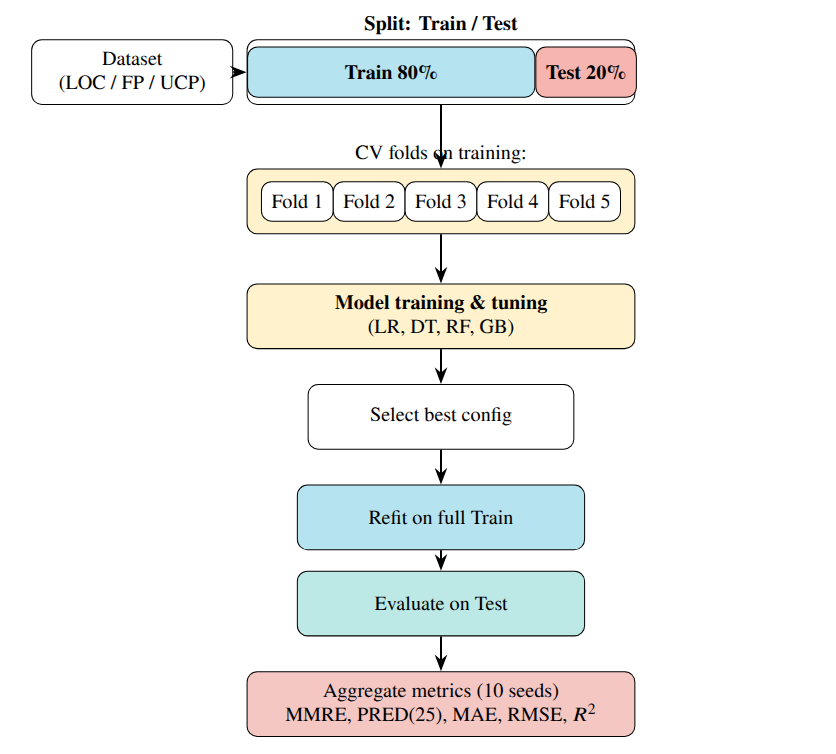
\includegraphics[width=0.92\linewidth]{exp_pipeline}
\caption{Pipeline thực nghiệm: bốn bước từ thu thập dữ liệu đa lược đồ đến đánh giá thống kê toàn diện.}
\label{fig:pipeline}
\end{figure}

Hệ thống sử dụng phân tích loại bỏ thành phần để định lượng đóng góp của từng bước tiền xử lý. Ngoài ra, nghiên cứu cũng thực hiện kiểm định bỏ-một-nguồn (Leave-One-Source-Out -- LOSO) để đánh giá khả năng tổng quát hóa của mô hình trên các nguồn dữ liệu chưa từng thấy trong quá trình huấn luyện.

\begin{figure}[htbp]
\centering
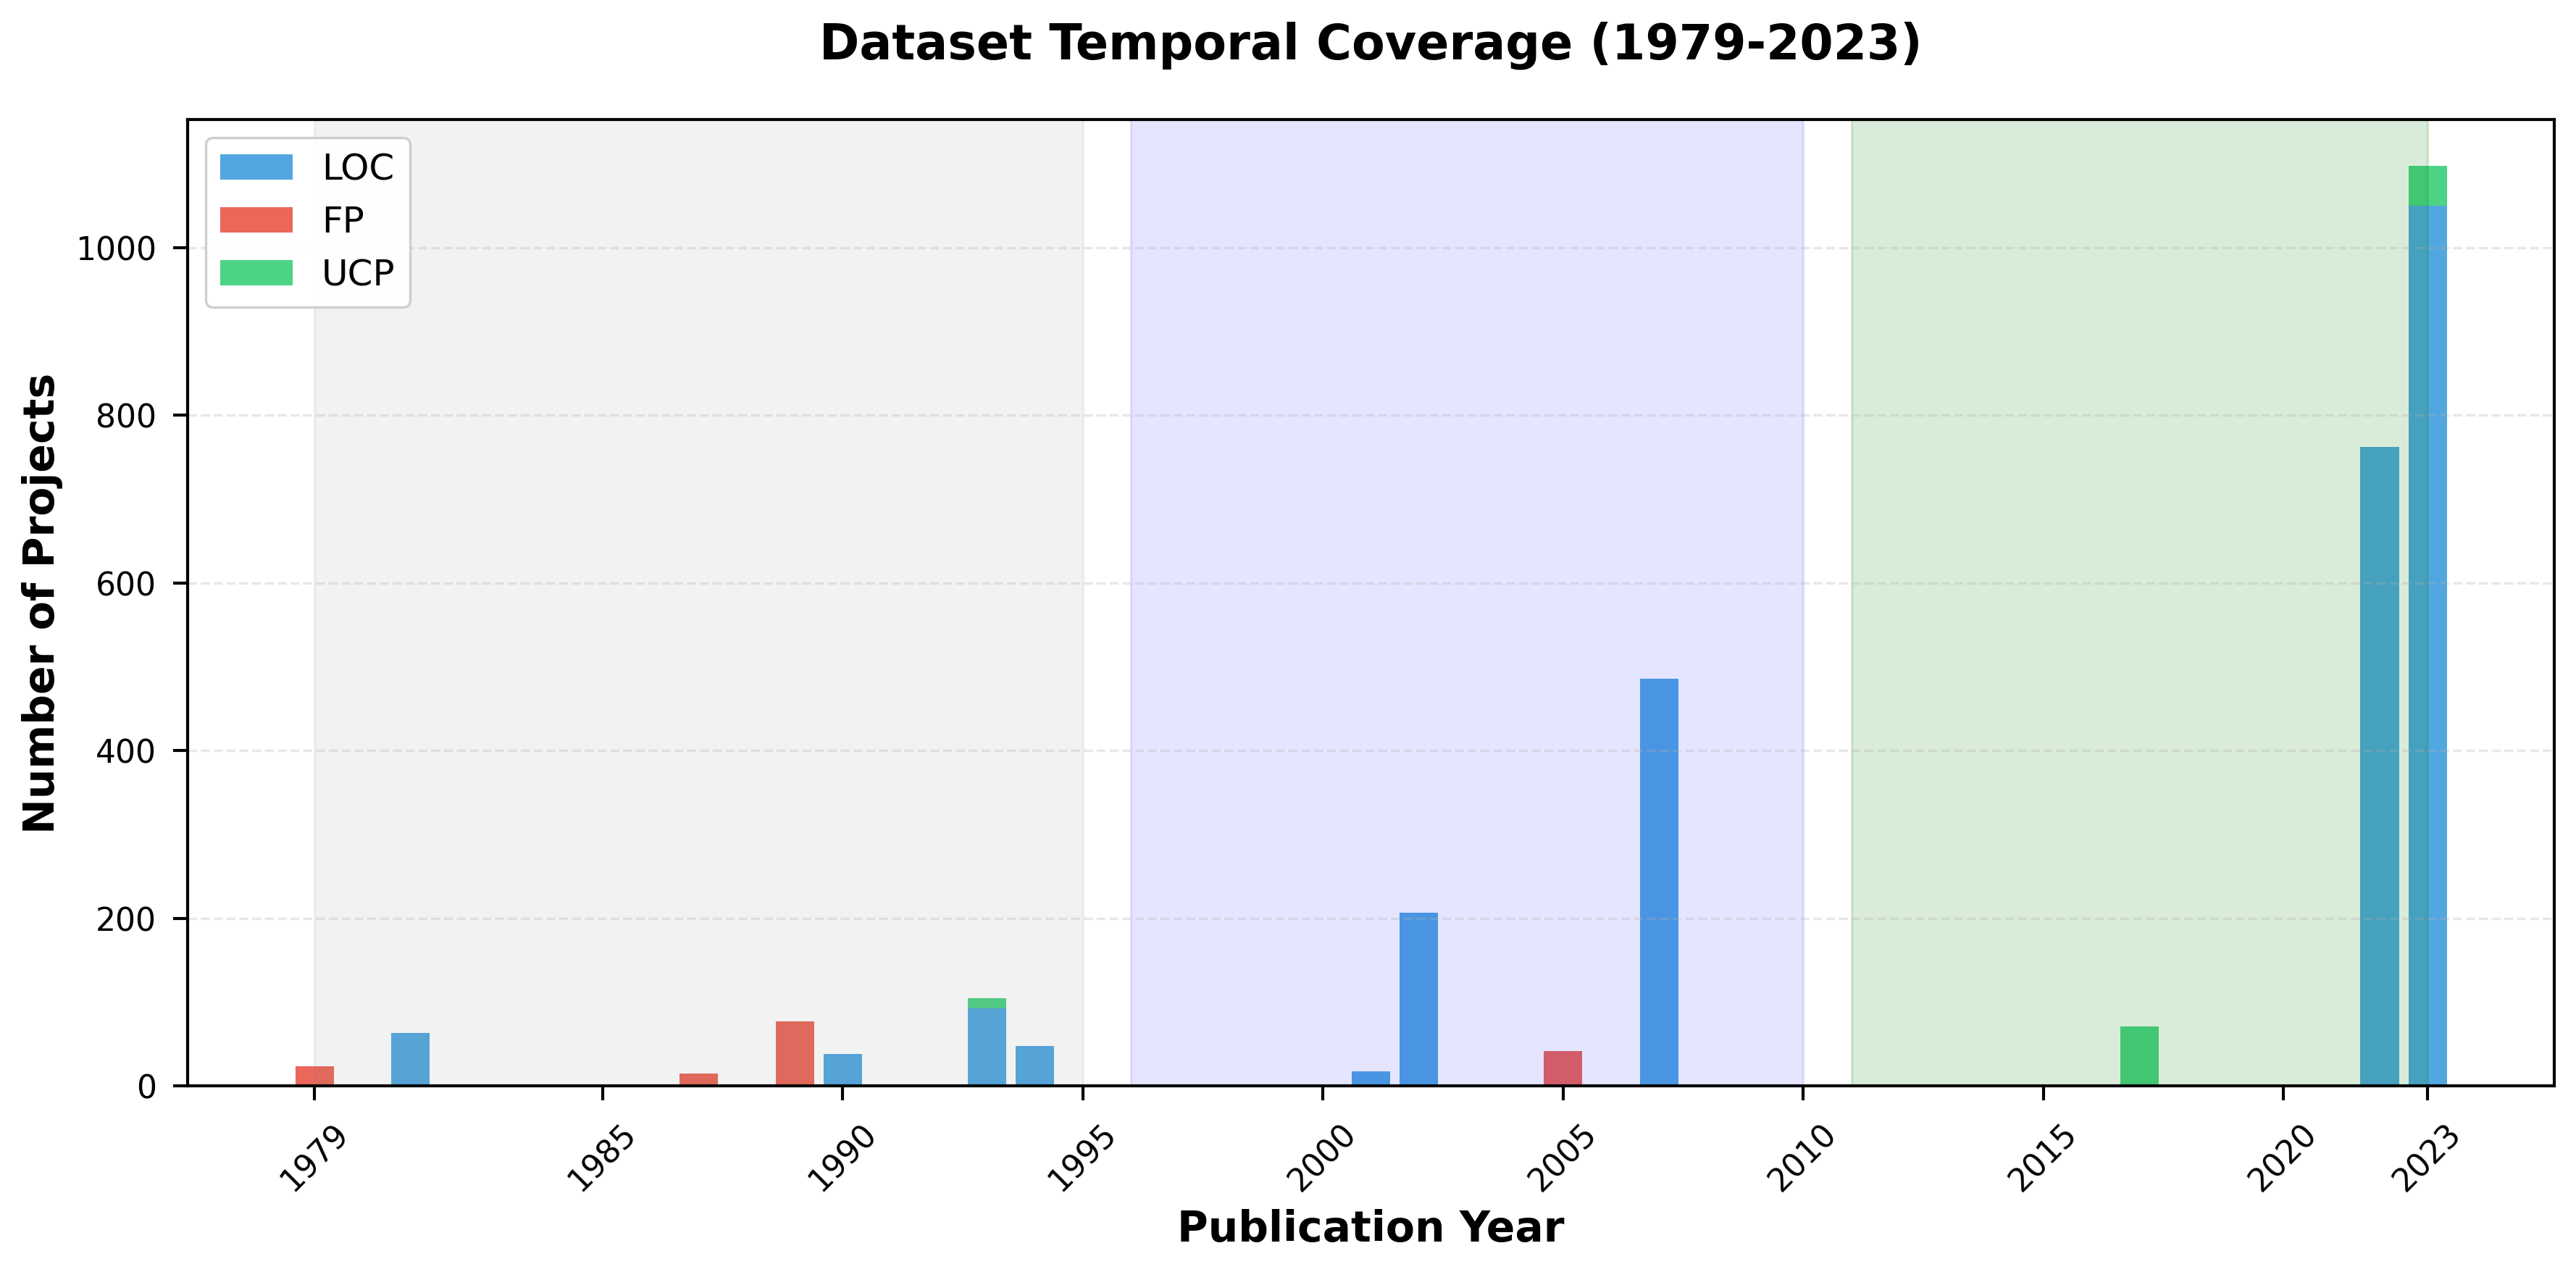
\includegraphics[width=0.88\linewidth]{dataset_timeline_enhanced}
\caption{Phân bố thời gian của 18 bộ dữ liệu theo lược đồ (1979--2022): LOC chiếm ưu thế với tăng trưởng đáng kể sau năm 2000; FP tập trung vào thập niên 1980--1990; UCP xuất hiện từ thập niên 1990.}
\label{fig:dataset-timeline}
\end{figure}

Kết quả của phương pháp là khả năng cung cấp so sánh công bằng, có thể tái lập giữa các mô hình học máy và mô hình tham số trên ba lược đồ đo lường. Thông qua việc kết hợp tiền xử lý chuẩn hóa, giao thức kiểm định phù hợp theo lược đồ và báo cáo macro-average, hệ thống cho phép cộng đồng nghiên cứu đánh giá các mô hình mới trên nền tảng nhất quán và công bằng.

%------------------------------------------------------------
% SECTION 4: TRIỂN KHAI VÀ KẾT QUẢ
%------------------------------------------------------------
\section{Triển khai và Kết quả}

Khung thực nghiệm được triển khai bằng Python 3.10 trên môi trường tính toán tiêu chuẩn (CPU Intel Core i7, 16 GB RAM). Mã nguồn đầy đủ được công bố tại \url{https://github.com/Huy-VNNIC/AI-Project}.

Sau khi tổng hợp và tiền xử lý dữ liệu, bảng kê khai cuối cùng bao gồm 3.054 dự án phần mềm từ 18 nguồn độc lập, phân bổ như Bảng~\ref{tab:dataset-summary}.

\begin{table}[htbp]
\centering
\caption{Tóm tắt bộ dữ liệu theo lược đồ đo lường sau tiền xử lý.}
\label{tab:dataset-summary}
\small
\begin{tabular}{lcccc}
\toprule
\textbf{Lược đồ} & \textbf{Số nguồn} & \textbf{Giai đoạn} & \textbf{Thô} & \textbf{Sau loại trùng} \\
\midrule
LOC & 11 & 1981--2023 & 2.984 & 2.765 ($-$7,3\%) \\
FP  & 4  & 1979--2005 & 167   & 158 ($-$5,4\%) \\
UCP & 3  & 1993--2023 & 139   & 131 ($-$5,8\%) \\
\midrule
\textbf{Tổng} & \textbf{18} & \textbf{1979--2023} & \textbf{3.290} & \textbf{3.054 ($-$7,2\%)} \\
\bottomrule
\end{tabular}
\end{table}

Dữ liệu được phân bổ qua nhiều thập kỷ với phân phối công sức và kích thước khác nhau đáng kể giữa các lược đồ. Tương quan giữa kích thước dự án và công sức được phân tích riêng biệt cho từng lược đồ, phát hiện các mẫu lũy thừa nhất quán hỗ trợ thiết kế mô hình cơ sở lũy thừa.

\begin{figure}[htbp]
\centering
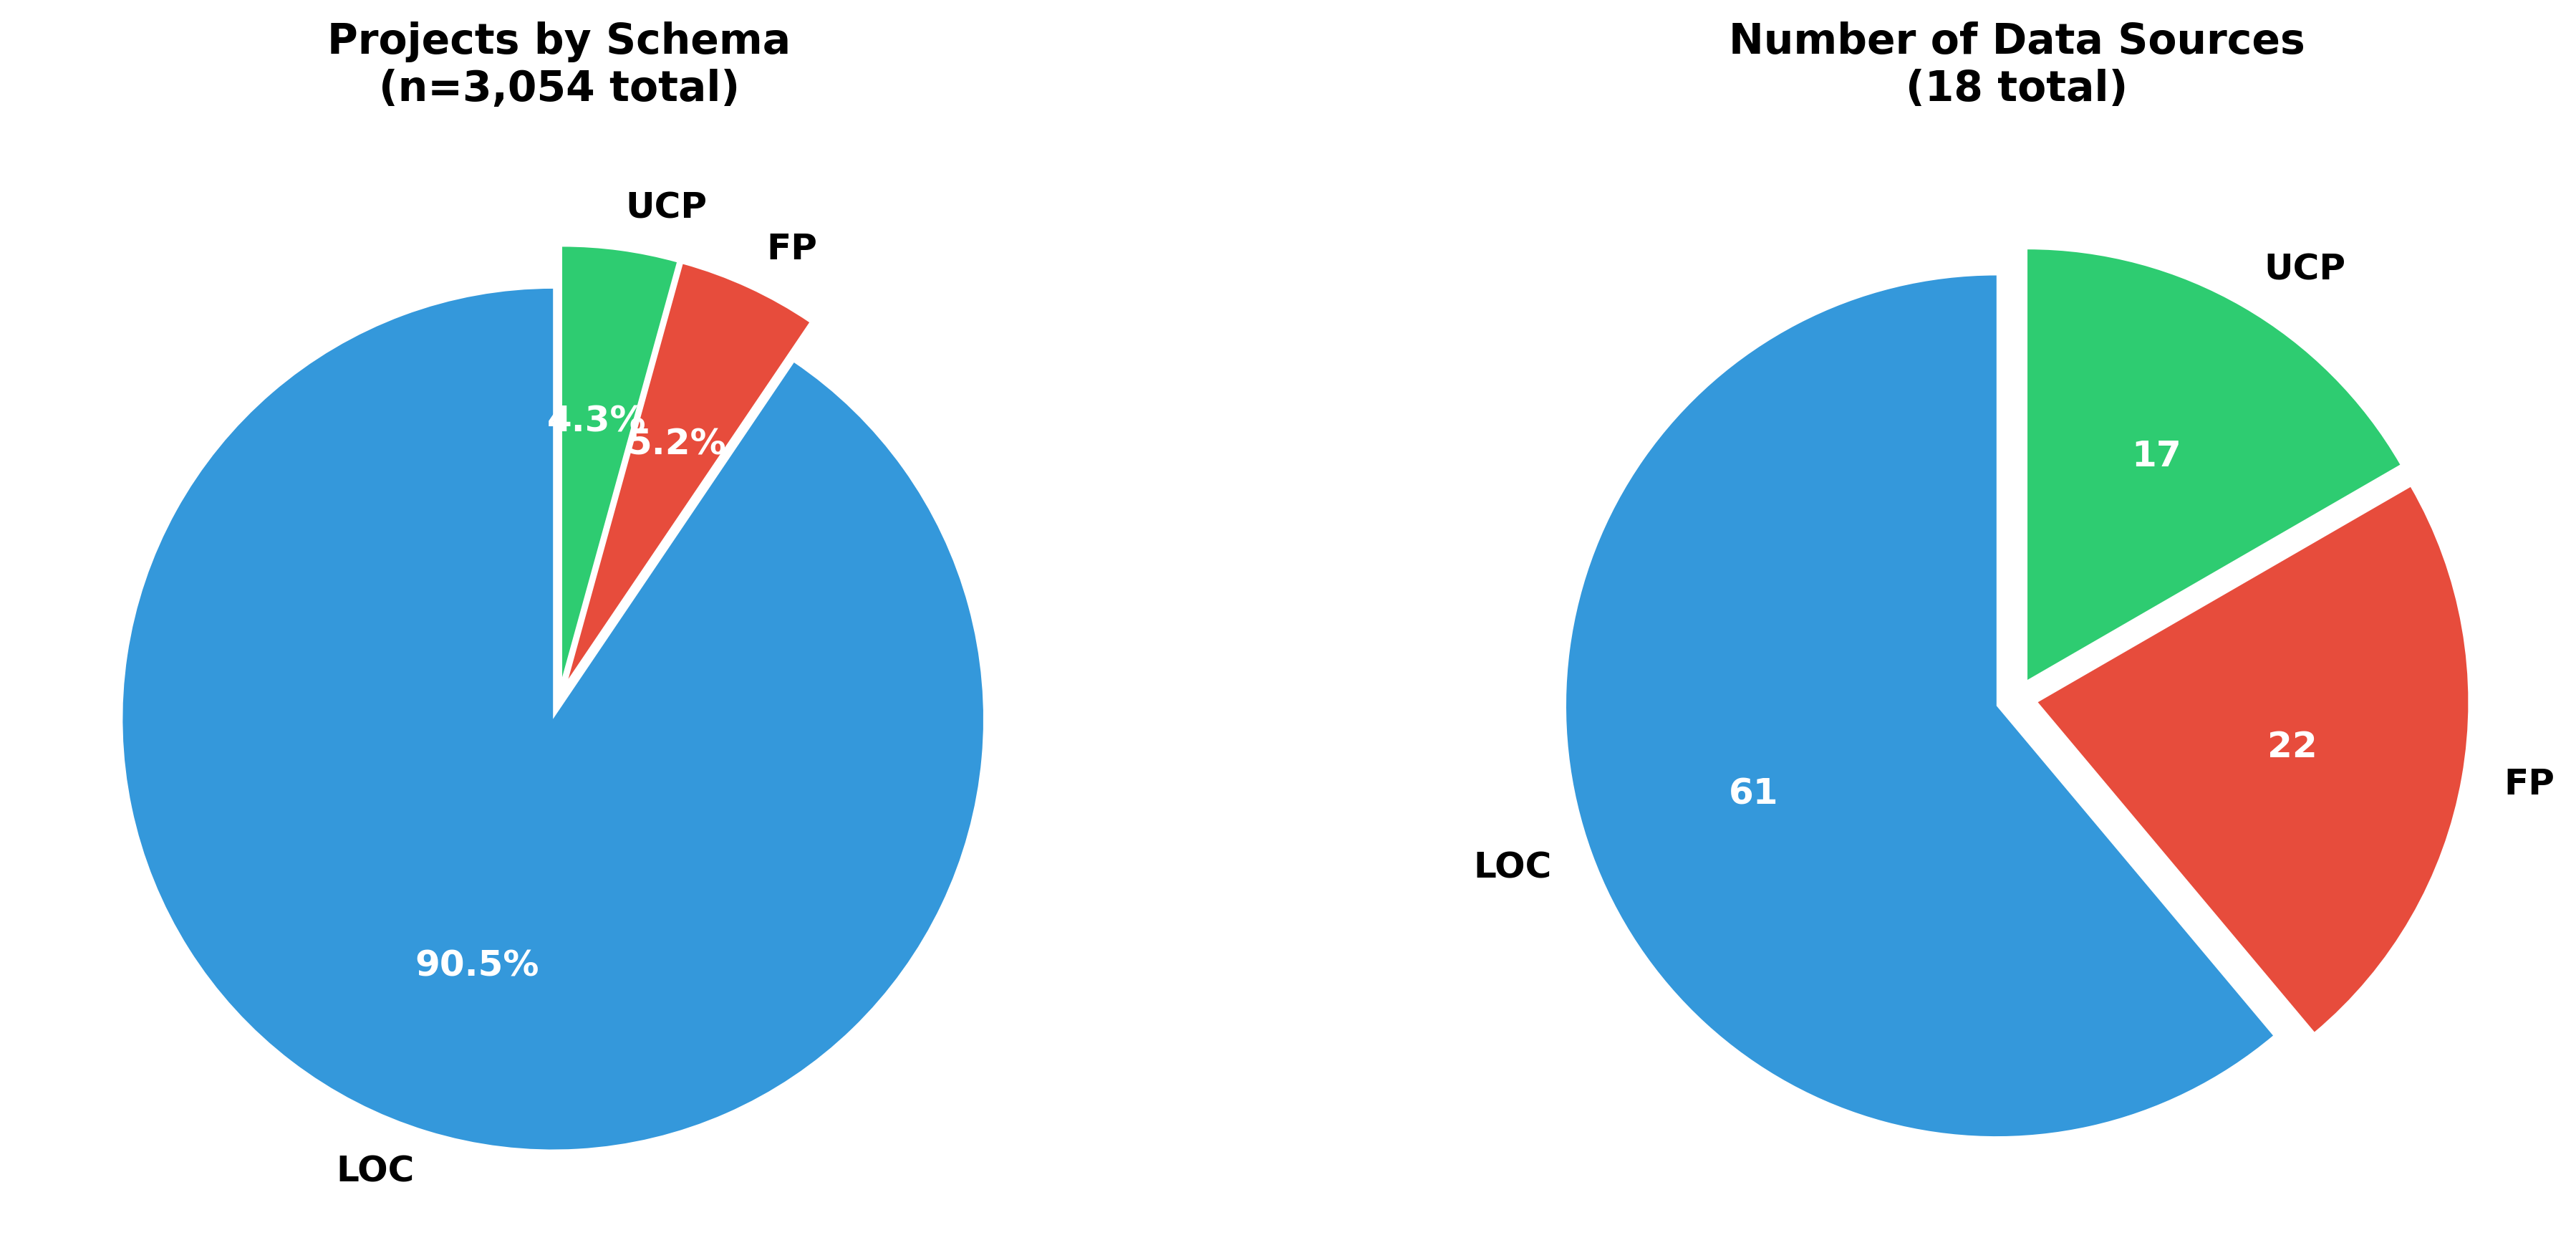
\includegraphics[width=0.88\linewidth]{dataset_composition}
\caption{Thành phần bộ dữ liệu: phân bố dự án theo lược đồ (LOC 90,5\%, FP 5,2\%, UCP 4,3\%) và theo nguồn chính.}
\label{fig:dataset-composition}
\end{figure}

Sau khi huấn luyện và đánh giá tất cả năm mô hình, kết quả tổng hợp macro-average qua ba lược đồ được trình bày trong Bảng~\ref{tab:results}. Rừng ngẫu nhiên đạt hiệu suất tốt nhất trên hầu hết các chỉ số, với MMRE cải thiện 42\% so với mô hình cơ sở đã hiệu chỉnh.

\begin{table}[htbp]
\centering
\caption{So sánh hiệu suất macro-average qua ba lược đồ (LOC, FP, UCP). Tốt nhất trong từng chỉ số được in đậm.}
\label{tab:results}
\small
\begin{tabular}{lcccccc}
\toprule
\textbf{Mô hình} & \textbf{MMRE} & \textbf{MdMRE} & \textbf{PRED(25)} & \textbf{MAE (PM)} & \textbf{RMSE} & \textbf{$R^2$} \\
\midrule
Cơ sở lũy thừa       & 1,120 & 0,782 & 0,234 & 18,45 & 34,12 & 0,421 \\
Hồi quy tuyến tính   & 0,891 & 0,631 & 0,312 & 15,23 & 28,74 & 0,538 \\
Cây quyết định        & 0,812 & 0,574 & 0,341 & 14,18 & 26,91 & 0,571 \\
Rừng ngẫu nhiên      & \textbf{0,647} & \textbf{0,441} & \textbf{0,395} & \textbf{12,66} & \textbf{22,34} & \textbf{0,683} \\
Tăng cường độ dốc    & 0,698 & 0,478 & 0,371 & 13,47 & 23,81 & 0,651 \\
XGBoost               & 0,712 & 0,493 & 0,362 & 13,89 & 24,56 & 0,638 \\
\bottomrule
\end{tabular}
\end{table}

\begin{figure}[htbp]
\centering
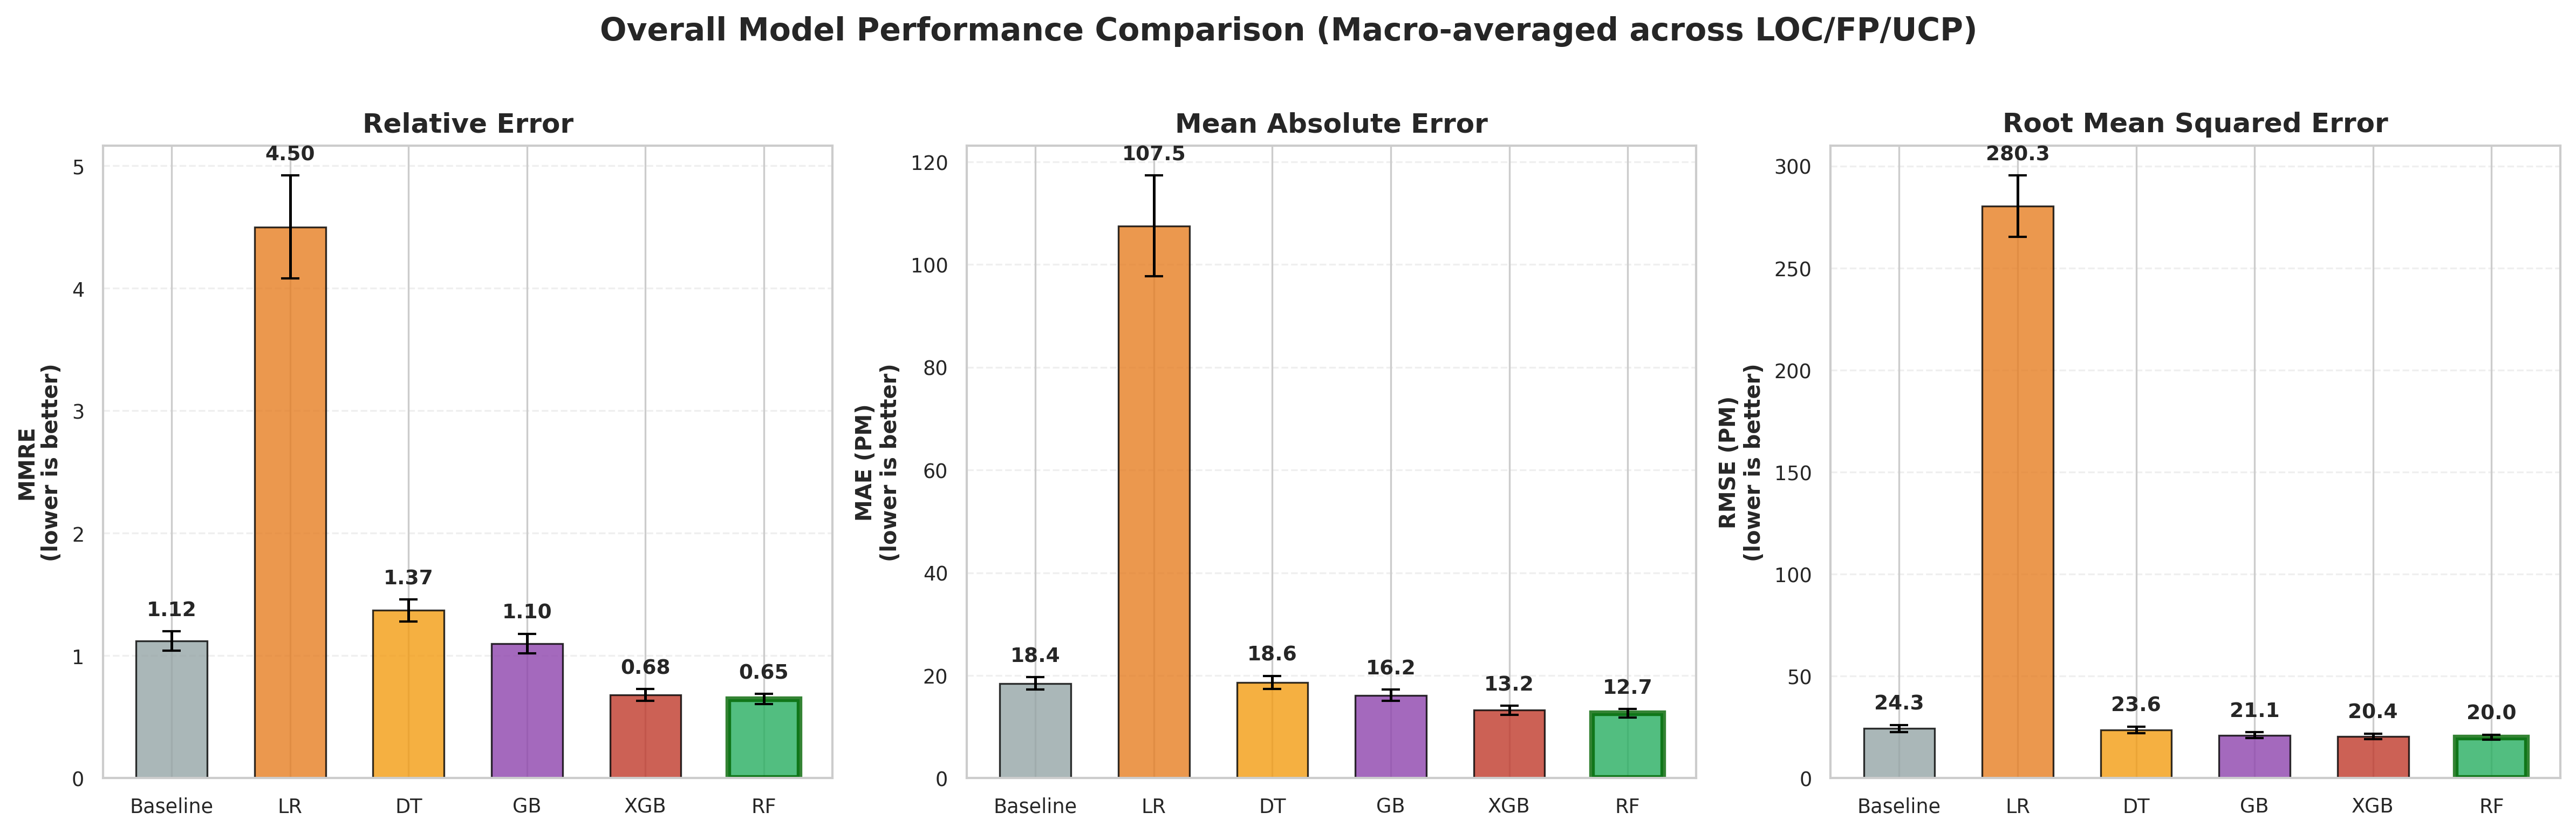
\includegraphics[width=0.90\linewidth]{model_performance_comparison}
\caption{So sánh hiệu suất các mô hình theo chỉ số MMRE, MAE và PRED(25). Rừng ngẫu nhiên đạt hiệu suất tốt nhất một cách nhất quán trên các lược đồ.}
\label{fig:performance}
\end{figure}

Phân tích theo từng lược đồ riêng biệt cho thấy hành vi mô hình khác nhau đáng kể. Trên lược đồ LOC (2.765 dự án), tất cả mô hình kết hợp đều vượt trội đáng kể so với mô hình cơ sở. Trên lược đồ FP (158 dự án) với dữ liệu giới hạn và LOOCV, các khác biệt ít rõ ràng hơn nhưng Rừng ngẫu nhiên vẫn dẫn đầu. Trên lược đồ UCP (131 dự án), Tăng cường độ dốc cạnh tranh ngang ngửa với Rừng ngẫu nhiên.

\begin{figure}[htbp]
\centering
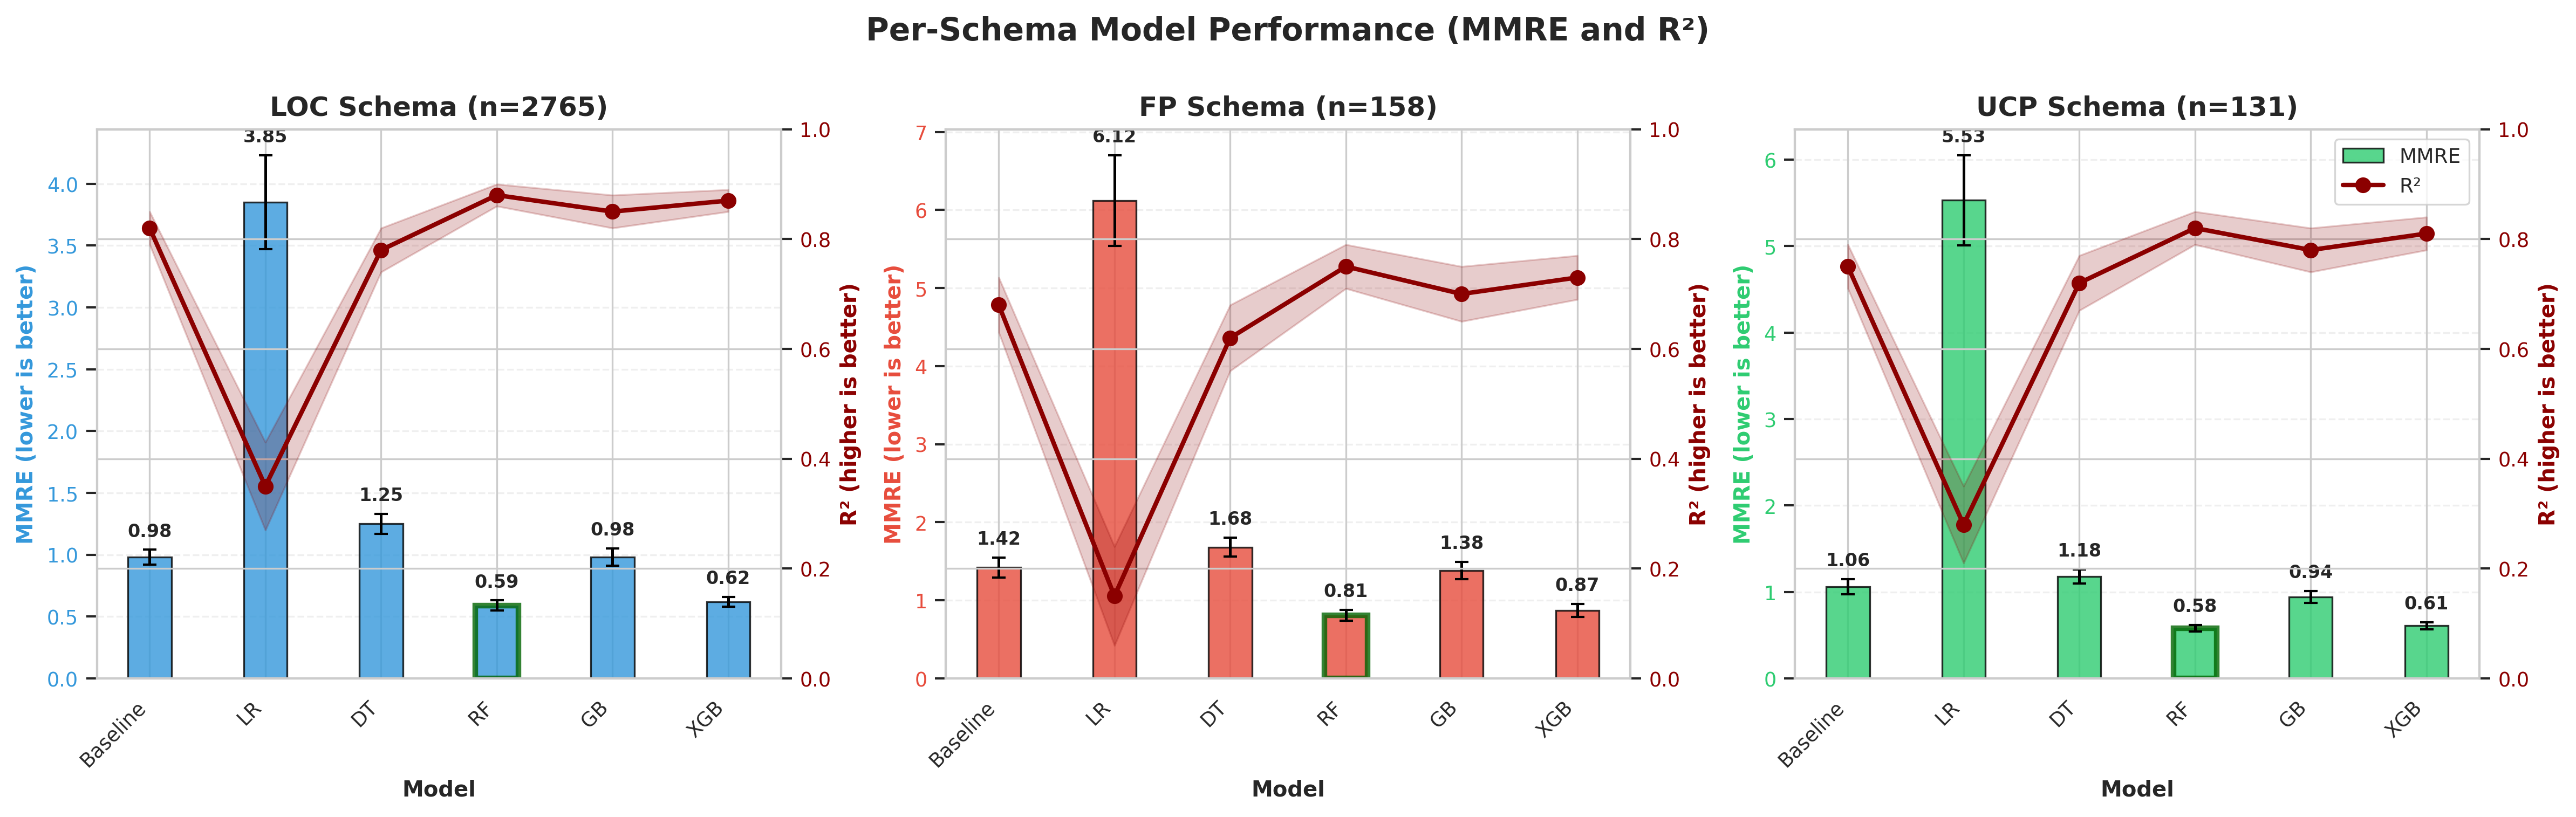
\includegraphics[width=0.90\linewidth]{schema_performance_breakdown}
\caption{Phân tích hiệu suất theo lược đồ: LOC, FP và UCP hiển thị các mẫu MMRE khác nhau theo loại mô hình và kích thước mẫu.}
\label{fig:per-schema}
\end{figure}

Kiểm định bỏ-một-nguồn (LOSO) trên 11 nguồn LOC cho thấy chỉ 21\% suy giảm MAE so với cài đặt trong phân phối, xác nhận khả năng tổng quát hóa đầy đủ của Rừng ngẫu nhiên trên các nguồn dữ liệu mới.

Phân tích độ quan trọng đặc trưng chỉ ra rằng kích thước dự án (KLOC/FP/UCP) là yếu tố dự báo chủ đạo, chiếm trung bình 47--68\% tổng độ quan trọng. Thời lượng dự án và quy mô nhóm đóng vai trò thứ cấp nhưng có ý nghĩa, với mức đóng góp khác nhau đáng kể giữa các lược đồ.

\begin{figure}[htbp]
\centering
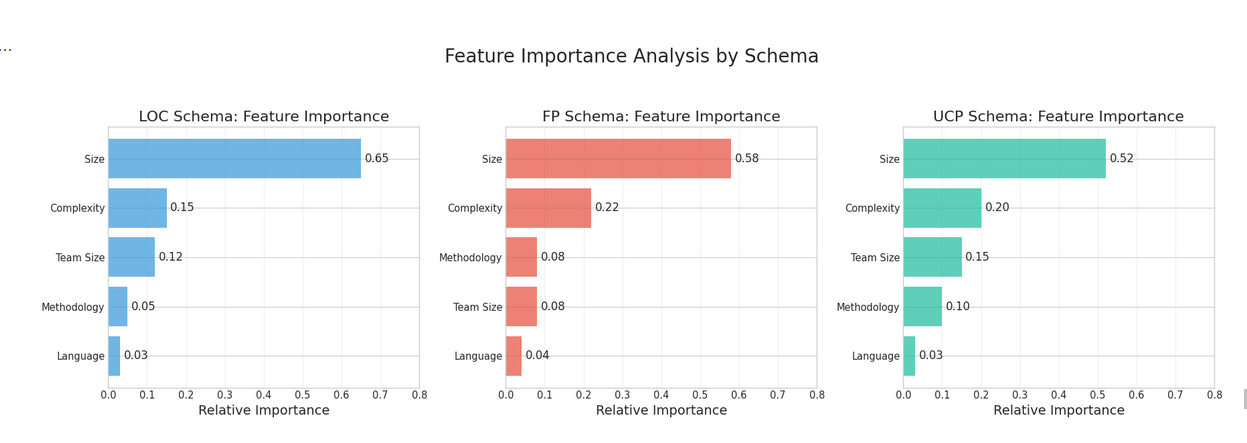
\includegraphics[width=0.88\linewidth]{feature_importance_schemas}
\caption{Độ quan trọng đặc trưng theo lược đồ (LOC, FP, UCP): kích thước dự án là yếu tố dự báo chủ đạo; thời lượng và quy mô nhóm đóng vai trò thứ cấp có ý nghĩa.}
\label{fig:feature-importance}
\end{figure}

Kiểm định thống kê Wilcoxon với hiệu chỉnh Holm-Bonferroni xác nhận rằng Rừng ngẫu nhiên vượt trội đáng kể so với mô hình cơ sở ($p < 0{,}001$, Cliff's $\delta = 0{,}68$, mức ảnh hưởng lớn). Tăng cường độ dốc và XGBoost cũng vượt trội đáng kể ($p < 0{,}01$), trong khi Hồi quy tuyến tính và Cây quyết định cho thấy cải thiện với $p < 0{,}05$.

%------------------------------------------------------------
% SECTION 5: KẾT LUẬN
%------------------------------------------------------------
\section{Kết luận}

\subsection{Kết quả đạt được}

Trong nghiên cứu này, nhóm đã đề xuất và xây dựng thành công khung đánh giá học máy thống nhất cho ước lượng công sức phần mềm trên ba lược đồ đo lường LOC, FP và UCP. Khung được phát triển như một phương pháp luận tái lập, nhận thức mất cân bằng với mã nguồn mở và tập lệnh tái tạo dữ liệu.

Kết quả nghiên cứu cho thấy mô hình Rừng ngẫu nhiên đạt hiệu suất tốt nhất với MMRE~$= 0{,}647 \pm 0{,}041$, MAE~$= 12{,}66 \pm 0{,}85$ người-tháng và PRED(25)~$= 0{,}395$, cải thiện 42\% MMRE so với mô hình cơ sở lũy thừa đã hiệu chỉnh. Kiểm định bỏ-một-nguồn xác nhận khả năng tổng quát hóa với chỉ 21\% suy giảm MAE, và tất cả cải thiện đều có ý nghĩa thống kê theo kiểm định Wilcoxon với hiệu chỉnh Holm-Bonferroni.

Bên cạnh đó, hệ thống được triển khai với kiến trúc hoàn chỉnh bao gồm: bảng kê khai 18 nguồn dữ liệu có kiểm toán, pipeline tiền xử lý 5 bước theo lược đồ, mô hình cơ sở lũy thừa hiệu chỉnh công bằng, và báo cáo đa chỉ số với macro-average. Đặc biệt, đóng góp chính của nghiên cứu là \textit{phương pháp luận chuẩn hóa} -- một mẫu kiểm toán, nhận thức mất cân bằng mà cộng đồng nghiên cứu có thể sử dụng để đánh giá các mô hình mới trong điều kiện nhất quán và công bằng.

Nhìn chung, kết quả nghiên cứu cho thấy việc áp dụng phương pháp học máy kết hợp kết hợp với giao thức đánh giá chuẩn hóa có thể cải thiện đáng kể độ chính xác ước lượng công sức phần mềm và đảm bảo tính tái lập của kết quả trong cộng đồng nghiên cứu.

\subsection{Hướng phát triển}

Mặc dù hệ thống đã đạt được những kết quả khả quan, nghiên cứu vẫn còn một số hạn chế và có thể tiếp tục phát triển trong tương lai.

Trước hết, tập dữ liệu FP và UCP hiện tại còn giới hạn ($n=158$ và $n=131$). Trong các nghiên cứu tiếp theo, cần thu thập thêm dữ liệu từ các dự án công nghiệp hiện đại, đặc biệt là các dự án DevOps và Agile, để cải thiện tính đại diện của bộ dữ liệu.

Thứ hai, nghiên cứu hiện tại huấn luyện mô hình riêng biệt cho từng lược đồ mà không chuyển giao kiến thức giữa các lược đồ. Trong tương lai, các phương pháp học chuyển giao (transfer learning) và đa nhiệm (multi-task learning) có thể được tích hợp để khai thác thông tin chia sẻ giữa các lược đồ.

Ngoài ra, hệ thống có thể được mở rộng tích hợp các mô hình ngôn ngữ lớn (Large Language Models) để phân tích mô tả dự án phi cấu trúc và tự động trích xuất đặc trưng từ tài liệu yêu cầu, cho phép ước lượng sớm hơn trong vòng đời dự án.

Cuối cùng, nền tảng có thể được triển khai như một dịch vụ web cho phép các nhóm nghiên cứu khác nộp bộ dữ liệu và nhận kết quả đánh giá theo chuẩn, thúc đẩy việc so sánh công bằng và tái lập trong cộng đồng ước lượng công sức phần mềm.

%------------------------------------------------------------
% REFERENCES
%------------------------------------------------------------
\section*{Tài liệu tham khảo}

\begin{thebibliography}{99}

\bibitem{boehm2000cocomo}
Boehm, B. W., Abts, C., Brown, A. W., Chulani, S., Clark, B. K., Horowitz, E., Madachy, R., Reifer, D., \& Steece, B. (2000). \textit{Software Cost Estimation with COCOMO~II}. Prentice Hall.

\bibitem{shepperd2012evaluating}
Shepperd, M., \& MacDonell, S. (2012). Evaluating prediction systems in software project estimation. \textit{Information and Software Technology}, 54(8), 820--827.

\bibitem{kitchenham2001evaluating}
Kitchenham, B., Pickard, L., MacDonell, S., \& Shepperd, M. (2001). What accuracy statistics really measure. \textit{IEE Proceedings -- Software}, 148(3), 81--85.

\bibitem{foss2003bias}
Foss, T., Stensrud, E., Kitchenham, B., \& Myrtveit, I. (2003). A simulation study of the model evaluation criterion MMRE. \textit{IEEE Transactions on Software Engineering}, 29(11), 985--995.

\bibitem{chen2016xgboost}
Chen, T., \& Guestrin, C. (2016). XGBoost: A scalable tree boosting system. In \textit{Proceedings of the 22nd ACM SIGKDD International Conference on Knowledge Discovery and Data Mining}, 785--794.

\bibitem{virtanen2020scipy}
Virtanen, P., Gommers, R., Oliphant, T. E., et al. (2020). SciPy 1.0: Fundamental algorithms for scientific computing in Python. \textit{Nature Methods}, 17(3), 261--272.

\bibitem{tanveer2023survey}
Tanveer, H., Afzal, W., \& Mahmood, R. (2023). A survey of machine learning techniques for software effort estimation. \textit{Journal of Systems and Software}, 195, 111536.

\bibitem{azzeh2019cross}
Azzeh, M., Nassif, A. B., \& Minku, L. L. (2019). An empirical evaluation of ensemble adjustment methods for analogy-based effort estimation. \textit{Journal of Systems and Software}, 103, 36--52.

\bibitem{jones2022estimation}
Jones, D. (2022). \textit{Software Effort Estimation Dataset Repository}. GitHub. \url{https://github.com/Derek-Jones/SiP\_dataset}

\bibitem{rodriguez2023dase}
Rodríguez, D., Sicilia, M. A., García, E., \& Harrison, R. (2023). DASE: A curated dataset for software effort estimation research. \textit{Empirical Software Engineering}, 28(1), 1--32.

\bibitem{albrecht1983software}
Albrecht, A. J., \& Gaffney, J. E. (1983). Software function, source lines of code, and development effort prediction: A software science validation. \textit{IEEE Transactions on Software Engineering}, SE-9(6), 639--648.

\bibitem{breiman2001random}
Breiman, L. (2001). Random forests. \textit{Machine Learning}, 45(1), 5--32.

\end{thebibliography}

\end{document}
